\documentclass[a4paper, 11pt, notitlepage, english]{article}

\usepackage{babel}
\usepackage[utf8]{inputenc}
\usepackage[T1]{fontenc, url}
\usepackage{textcomp}
\usepackage{amsmath, amssymb}
\usepackage{amsbsy, amsfonts}
\usepackage{graphicx, color, xcolor}
\usepackage{verbatim, listings, fancyvrb}
\usepackage{parskip}
\usepackage{framed}
\usepackage{amsmath}
\usepackage{multicol}
\usepackage{url}
\usepackage{flafter}
\usepackage{simplewick}
\usepackage{amsthm}
\usepackage{bbold}


\usepackage{caption}
\DeclareCaptionLabelSeparator{colon}{. }
\renewcommand{\captionfont}{\small\sffamily}
\renewcommand{\captionlabelfont}{\bf\sffamily}
\usepackage{float}
%\floatstyle{ruled}
%\restylefloat{figure}
\setlength{\captionmargin}{20pt}
%\addto\captionsenglish{\renewcommand{\figurename}{Fig.}}
\usepackage{bigstrut}
\setlength{\tabcolsep}{12pt}


\newtheorem{theorem}[]{Wick's Theorem}[]

\DeclareUnicodeCharacter{00A0}{~}

\definecolor{javared}{rgb}{0.6,0,0} % for strings
\definecolor{javagreen}{rgb}{0.25,0.5,0.35} % comments
\definecolor{javapurple}{rgb}{0.5,0,0.35} % keywords
\definecolor{javadocblue}{rgb}{0.25,0.35,0.75} % javadoc

\lstset{language=python,
basicstyle=\ttfamily\scriptsize,
keywordstyle=\color{javapurple},%\bfseries,
stringstyle=\color{javared},
commentstyle=\color{javagreen},
morecomment=[s][\color{javadocblue}]{/**}{*/},
morekeywords={super, with},
% numbers=left,
% numberstyle=\tiny\color{black},
stepnumber=2,
numbersep=10pt,
tabsize=2,
showspaces=false,
captionpos=b,
showstringspaces=false,
frame= single,
breaklines=true}

\usepackage{geometry}
\geometry{headheight=0.01mm}
\geometry{top=20mm, bottom=20mm, left=34mm, right=34mm}

\renewcommand{\arraystretch}{2}
\setlength{\tabcolsep}{10pt}
\makeatletter
\renewcommand*\env@matrix[1][*\c@MaxMatrixCols c]{%
  \hskip -\arraycolsep
  \let\@ifnextchar\new@ifnextchar
  \array{#1}}
%
% Definering av egne kommandoer og miljøer
%
\newcommand{\dd}[1]{\ \text{d}#1}
\newcommand{\f}[2]{\frac{#1}{#2}} 
\newcommand{\beq}{\begin{equation}}
\newcommand{\eeq}{\end{equation}}
\newcommand{\bra}[1]{\langle #1|}
\newcommand{\ket}[1]{|#1 \rangle}
\newcommand{\braket}[2]{\langle #1 | #2 \rangle}
\newcommand{\brakket}[2]{\langle #1 || #2 \rangle}
\newcommand{\braup}[1]{\langle #1 \left|\uparrow\rangle\right.}
\newcommand{\bradown}[1]{\langle #1 \left|\downarrow\rangle\right.}
\newcommand{\av}[1]{\left| #1 \right|}
\newcommand{\op}[1]{\hat{#1}}
\newcommand{\braopket}[3]{\langle #1 | {#2} | #3 \rangle}
\newcommand{\ketbra}[2]{\ket{#1}\bra{#2}}
\newcommand{\pp}[1]{\frac{\partial}{\partial #1}}
\newcommand{\ppn}[1]{\frac{\partial^2}{\partial #1^2}}
\newcommand{\up}{\left|\uparrow\rangle\right.}
\newcommand{\upup}{\left|\uparrow\uparrow\rangle\right.}
\newcommand{\down}{\left|\downarrow\rangle\right.}
\newcommand{\downdown}{\left|\downarrow\downarrow\rangle\right.}
\newcommand{\updown}{\left|\uparrow\downarrow\rangle\right.}
\newcommand{\downup}{\left|\downarrow\uparrow\rangle\right.}
\newcommand{\bupup}{\left.\langle\uparrow\uparrow\right|}
\newcommand{\bdowndown}{\left.\langle\downarrow\downarrow\right|}
\newcommand{\bupdown}{\left.\langle\uparrow\downarrow\right|}
\newcommand{\bdownup}{\left.\langle\downarrow\uparrow\right|}
\renewcommand{\d}{{\rm d}}
\newcommand{\Res}[2]{{\rm Res}(#1;#2)}
\newcommand{\To}{\quad\Rightarrow\quad}
\newcommand{\eps}{\epsilon}
\newcommand{\inner}[2]{\langle #1 , #2 \rangle}
\renewcommand{\u}{\uparrow}
\renewcommand{\d}{\downarrow}
\newcommand{\dddd}{\d\d\d\d}
\newcommand{\uddd}{\u\d\d\d}
\newcommand{\dudd}{\d\u\d\d}
\newcommand{\ddud}{\d\d\u\d}
\newcommand{\dddu}{\d\d\d\u}
\newcommand{\uudd}{\u\u\d\d}
\newcommand{\udud}{\u\d\u\d}
\newcommand{\uddu}{\u\d\d\u}
\newcommand{\duud}{\d\u\u\d}
\newcommand{\dudu}{\d\u\d\u}
\newcommand{\dduu}{\d\d\u\u}
\newcommand{\uuud}{\u\u\u\d}
\newcommand{\uudu}{\u\u\d\u}
\newcommand{\uduu}{\u\d\u\u}
\newcommand{\duuu}{\d\u\u\u}
\newcommand{\uuuu}{\u\u\u\u}
\newcommand{\m}{\text{-}}
\newcommand{\ui}{{\u_1}}
\newcommand{\uii}{{\u_2}}
\newcommand{\uiii}{{\u_3}}
\newcommand{\di}{{\d_1}}
\newcommand{\dii}{{\d_2}}
\newcommand{\diii}{{\d_3}}

\newenvironment{psmallmatrix}
  {\left(\begin{smallmatrix}}
  {\end{smallmatrix}\right)}

\newenvironment{bsmallmatrix}
  {\left[\begin{smallmatrix}}
  {\end{smallmatrix}\right]}



\newcommand{\bt}[1]{\boldsymbol{#1}}
\newcommand{\mat}[1]{\textsf{\textbf{#1}}}
\newcommand{\I}{\boldsymbol{\mathcal{I}}}
\newcommand{\p}{\partial}
%
% Navn og tittel
%
\author{Jonas van den Brink \\ \texttt{j.v.brink@fys.uio.no}}
\title{Second Midterm Project \\ FYS-KJM4480}

\begin{document}
\maketitle

\clearpage

\subsection*{Exercise 1)}
Show that $\op{H_0}$ and $V$ commute with $\op{S}_z$ and $\op{S}^2$.

\begin{align*}
	\op{H}_0 &:= \xi \sum_{p \sigma} (p-1)a_{p\sigma}^\dagger a_{p\sigma}, \\
	\op{V} &:= -\frac{1}{2}g \sum_{p q} a_{p+}^\dagger a_{p-}^\dagger a_{q-} a_{q+}, \\
	\op{S}_z &:= \frac{1}{2}\sum_{p\sigma} \sigma a_{p\sigma}^\dagger a_{p\sigma}, \\
	\op{S}^2 &:= \op{S}_z^2 + \frac{1}{2}\big(\op{S}_+\op{S}_- + \op{S}_-\op{S}_+\big), \\
	\op{S}_\pm &:= \sum_p a_{p\pm}^\dagger a_{p\mp}.
\end{align*}

Anti-commutation relations
$$\{\op{a}_\alpha^\dagger, \op{a}_\beta^\dagger \} = \{\op{a}_\alpha, \op{a}_\beta \} = 0, \qquad \{\op{a}_\alpha^\dagger, \op{a}_\beta \} = \delta_{\alpha\beta},$$

\subsubsection*{The commutator $[\op{H_0}, \op{S}_z]$}
We start by inserting the operators in the definition
\begin{align*}
[\op{H}_0, \op{S}_z] &= \op{H}_0\op{S}_z - \op{S}_z\op{H}_0 \\
&= \frac{\xi}{2}\sum_{pq \sigma\lambda} \lambda(p-1)\bigg(a_{p\sigma}^\dagger a_{p\sigma}  a_{q\lambda}^\dagger a_{q\lambda}
-   a_{q\lambda}^\dagger a_{q\lambda}  a_{p\sigma}^\dagger a_{p\sigma}\bigg).
\end{align*}
We now swap the two middle operators in the second term, this gives a delta-term
\begin{align*}
[\op{H}_0, \op{S}_z] &= \frac{\xi}{2}\sum_{pq \sigma\lambda} \lambda(p-1)\bigg(a_{p\sigma}^\dagger a_{p\sigma}  a_{q\lambda}^\dagger a_{q\lambda} 
-   a_{q\lambda}^\dagger \big(\delta_{pq}\delta_{\sigma\lambda} - a_{p\sigma}^\dagger a_{q\lambda} \big) a_{p\sigma}\bigg) \\
&= \frac{\xi}{2}\sum_{pq \sigma\lambda} \lambda(p-1)\bigg(a_{p\sigma}^\dagger a_{p\sigma}  a_{q\lambda}^\dagger a_{q\lambda}
+   a_{q\lambda}^\dagger a_{p\sigma}^\dagger a_{q\lambda} a_{p\sigma} - \delta_{pq}\delta_{\sigma\lambda}a_{q\lambda}^\dagger a_{p\sigma}
\bigg).
\end{align*}
We now swap the first and second, and third and fourth operator in the second term. We get no delta-terms, and we have no total change in sign
\begin{align*}
[\op{H}_0, \op{S}_z]  &= \frac{\xi}{2}\sum_{pq \sigma\lambda} \lambda(p-1)\bigg(a_{p\sigma}^\dagger a_{p\sigma}  a_{q\lambda}^\dagger a_{q\lambda}
+   a_{p\sigma}^\dagger  a_{q\lambda}^\dagger  a_{p\sigma} a_{q\lambda} - \delta_{pq}\delta_{\sigma\lambda}a_{q\lambda}^\dagger a_{p\sigma}
\bigg).
\end{align*}
Again we swap the two middle operators, getting another delta term
\begin{align*}
 [\op{H}_0, \op{S}_z]  &= \frac{\xi}{2}\sum_{pq \sigma\lambda} \lambda(p-1)\bigg(a_{p\sigma}^\dagger a_{p\sigma}  a_{q\lambda}^\dagger a_{q\lambda}
+  a_{p\sigma}^\dagger  \big(\delta_{pq}\delta_{\lambda\sigma} - a_{p\sigma} a_{q\lambda}^\dagger  \big) a_{q\lambda} - \delta_{pq}\delta_{\sigma\lambda}a_{q\lambda}^\dagger a_{p\sigma}
\bigg) \\
&= \frac{\xi}{2}\sum_{pq \sigma\lambda} \lambda(p-1) \delta_{pq}\delta_{\lambda\sigma}\big(a_{p\sigma}^\dagger a_{q\lambda} - a_{q\lambda}^\dagger a_{p\sigma}
\big).
\end{align*}
Due to the Kronecker-deltas the only surviving terms in the sums will have $p=q$ and $\sigma=\lambda$, meaning the two terms will cancel out, so we have
\begin{align*}
 [\op{H}_0, \op{S}_z] &= 0,
\end{align*}
and we have confirmed that $\op{H}_0$ and $\op{S}_z$ commute.

\clearpage

\subsubsection*{The commutator $[\op{V}, \op{S}_z]$}
Again, we start from the definition
\begin{align*}
[\op{V}, \op{S}_z] &= \op{V}\op{S}_z - \op{S}_z\op{V} \\
&= \frac{g}{4}\sum_{pqr\sigma} \sigma \bigg(a_{r\sigma}^\dagger a_{r\sigma} a_{p+}^\dagger a_{p-}^\dagger a_{q-} a_{q+} - a_{p+}^\dagger a_{p-}^\dagger a_{q-} a_{q+} a_{r\sigma}^\dagger a_{r\sigma} \bigg).
\end{align*}
We now move the $a_{r\sigma}^\dagger$-operator in the second term to the front by succesively swapping it to the left
\begin{align*}
a_{p+}^\dagger a_{p-}^\dagger &a_{q-} a_{q+} a_{r\sigma}^\dagger a_{r\sigma} \\ 
&= a_{p+}^\dagger a_{p-}^\dagger a_{q-} \big(\delta_{qr}\delta_{\sigma+} -  a_{r\sigma}^\dagger a_{q+} \big) a_{r\sigma} \\
&=\delta_{qr}\delta_{\sigma+} a_{p+}^\dagger a_{p-}^\dagger a_{q-} a_{r\sigma}  - a_{p+}^\dagger a_{p-}^\dagger \big(\delta_{qr}\delta_{\sigma-} -  a_{r\sigma}^\dagger a_{q-} \big) a_{q+} a_{r\sigma} \\
&=\delta_{qr}\delta_{\sigma+} a_{p+}^\dagger a_{p-}^\dagger a_{q-} a_{r\sigma}  - \delta_{qr}\delta_{\sigma-} a_{p+}^\dagger a_{p-}^\dagger a_{q+} a_{r\sigma} +  a_{r\sigma}^\dagger  a_{p+}^\dagger a_{p-}^\dagger a_{q-}  a_{q+} a_{r\sigma}.
\end{align*}
In the final term here, we now move the $a_{r\sigma}$ by successive shifts
\begin{align*}
a_{r\sigma}^\dagger  a_{p+}^\dagger & a_{p-}^\dagger a_{q-}  a_{q+} a_{r\sigma} \\
&= a_{r\sigma}^\dagger  a_{p+}^\dagger \big(\delta_{pr} \delta_{\sigma -} -  a_{r\sigma} a_{p-}^\dagger\big) a_{q-}  a_{q+} \\
&= \delta_{pr} \delta_{\sigma -} a_{r\sigma}^\dagger  a_{p+}^\dagger a_{q-}  a_{q+} -  a_{r\sigma}^\dagger  \big(\delta_{pr}\delta_{\sigma+} - a_{r\sigma}a_{p+}^\dagger\big) a_{p-}^\dagger a_{q-}  a_{q+} \\
&= \delta_{pr} \delta_{\sigma -} a_{r\sigma}^\dagger  a_{p+}^\dagger a_{q-}  a_{q+} -  \delta_{pr}\delta_{\sigma+} a_{r\sigma}^\dagger  a_{p-}^\dagger a_{q-}  a_{q+} + a_{r\sigma}^\dagger a_{r\sigma}a_{p+}^\dagger a_{p-}^\dagger a_{q-}  a_{q+}.\\
\end{align*}
Putting this result back into the original expression gives
\begin{align*}
[\op{V}, \op{S}_z] = \frac{g}{4}\sum_{pqr\sigma} \sigma \big(&
\delta_{pr}\delta_{\sigma+} a_{r\sigma}^\dagger  a_{p-}^\dagger a_{q-}  a_{q+}
+ \delta_{qr}\delta_{\sigma-} a_{p+}^\dagger a_{p-}^\dagger a_{q+} a_{r\sigma}\\[-0.3cm]
&\qquad- \delta_{qr}\delta_{\sigma+} a_{p+}^\dagger a_{p-}^\dagger a_{q-} a_{r\sigma}  
- \delta_{pr} \delta_{\sigma -} a_{r\sigma}^\dagger  a_{p+}^\dagger a_{q-}  a_{q+} \big).
\end{align*}
We now perform the sum over $\sigma$, giving
\begin{align*}
[\op{V}, \op{S}_z] = \frac{g}{4}\sum_{pqr} &
\delta_{pr} \big(a_{r+}^\dagger  a_{p-}^\dagger a_{q-}  a_{q+} + a_{r-}^\dagger a_{p+}^\dagger a_{q-}  a_{q+} \big) \\[-0.3cm]
&\qquad - \delta_{qr} \big( a_{p+}^\dagger a_{p-}^\dagger a_{q+} a_{r-} + a_{p+}^\dagger a_{p-}^\dagger a_{q-} a_{r+} \big).
\end{align*}
We now perform the sum over $p$ and $q$, we see the only surviving terms are those were $p=r$ or $q=r$, giving
\begin{align*}
[\op{V}, \op{S}_z] = \frac{g}{4}\sum_{r} \big(
a_{r+}^\dagger  a_{r-}^\dagger a_{r-}  a_{r+} + a_{r-}^\dagger a_{r+}^\dagger a_{r-}  a_{r+}  -  a_{r+}^\dagger a_{r-}^\dagger a_{r+} a_{r-} - a_{r+}^\dagger a_{r-}^\dagger a_{r-} a_{r+} \big).
\end{align*}
We see that the terms cancel each other out, leaving
\begin{align*}
 [\op{V}, \op{S}_z] &= 0,
\end{align*}
and we have confirmed that $\op{V}$ and $\op{S}_z$ commute.

\clearpage

\subsubsection*{The commutator $[\op{H_0}, \op{S}_\pm]$}
From the definition, we have
\begin{align*}
[\op{H}_0, \op{S}_\pm] &= \op{H}_0\op{S}_\pm - \op{S}_\pm\op{H}_0 \\
&= 
\xi \sum_{pq \sigma} (p-1) \big( a_{p\sigma}^\dagger a_{p\sigma}  a_{q\pm}^\dagger a_{q\mp}       
- a_{q\pm}^\dagger a_{q\mp} a_{p\sigma}^\dagger a_{p\sigma}\big).
\end{align*}
Again, we shift the operators around in the second term around, so that it cancels with the first term, we get the following result
\begin{align*}
[\op{H}_0, \op{S}_\pm] &= \xi \sum_{pq \sigma} (p-1) \delta_{pq} (\delta_{\sigma \pm} - \delta_{\sigma \mp}).
\end{align*}
We can now take the sum over $\sigma$, which makes the entire commutator vanish, as the two Kronecker-delta's with $\sigma $cancel each other out, so we have
\begin{align*}
[\op{H}_0, \op{S}_\pm] &= 0.
\end{align*}
And $\op{H}_0$ commutes with $\op{S}_\pm$.


\subsubsection*{The commutator $[\op{V}, \op{S}_\pm]$}
From the definition, we have
\begin{align*}
[\op{V}, \op{S}_\pm] &= \op{V}\op{S}_\pm - \op{S}_\pm\op{V} \\
&= -\frac{g}{2}\sum_{pqr} a_{p+}^\dagger a_{p-}^\dagger a_{q-} a_{q+} a_{r\pm}^\dagger a_{r\mp} - a_{r\pm}^\dagger a_{r\mp} a_{p+}^\dagger a_{p-}^\dagger a_{q-} a_{q+}.
\end{align*}
Shifting the operators around in the second term makes it cancel with the first, but shifting the operators generates some terms, we have
\begin{align*}
[\op{V}, \op{S}_\pm] &= \op{V}\op{S}_\pm - \op{S}_\pm\op{V} \\
&= \frac{g}{2}\sum_{pqr}
\big(\delta_{pr}\delta_{\mp +}  a_{r\pm}^\dagger a_{p-}^\dagger a_{q-} a_{q+}
- \delta_{pr}\delta_{\mp -} a_{r\pm}^\dagger a_{p+}^\dagger a_{q-} a_{q+} \\
&\qquad\qquad\qquad + \delta_{qr}\delta_{\pm -} a_{p+}^\dagger   a_{p-}^\dagger a_{q+} a_{r\mp}
- \delta_{qr} \delta_{\pm +}a_{p+}^\dagger   a_{p-}^\dagger a_{q-} a_{r\mp}\big).
\end{align*}
Summing over $p$ and $q$ gives
\begin{align*}
[\op{V}, \op{S}_\pm] &= \op{V}\op{S}_\pm - \op{S}_\pm\op{V} \\
&= \frac{g}{2}\sum_{r}
\big(\delta_{\mp +} a_{r\pm}^\dagger a_{r-}^\dagger a_{r-} a_{r+}
- \delta_{\mp -} a_{r\pm}^\dagger a_{r+}^\dagger a_{r-} a_{r+} \\
&\qquad\qquad\qquad + \delta_{\pm -} a_{r+}^\dagger   a_{r-}^\dagger a_{r+} a_{r\mp}
-  \delta_{\pm +}a_{r+}^\dagger   a_{r-}^\dagger a_{r-} a_{r\mp}\big).
\end{align*}

For top
\begin{align*}
-a_{r+}^\dagger a_{r+}^\dagger a_{r-} a_{r+} - a_{r+}^\dagger   a_{r-}^\dagger a_{r-} a_{r-}. \\
a_{r-}^\dagger a_{r-}^\dagger a_{r-} a_{r+} + a_{r+}^\dagger   a_{r-}^\dagger a_{r+} a_{r+}
\end{align*}

\section{THIS MUST BE FIXED}

\clearpage

\subsubsection*{The commutator $[\op{H}_0, \op{S}^2]$}

To compute the commutator between $\op{H}_0$ and $\op{S}^2$ we express the total spin by the operators $\op{S}_z$ and $\op{S}_\pm$, so we get
\begin{align*}
[\op{H}_0, \op{S}^2] &= [\op{H}_0, \op{S}_z^2 + \frac{1}{2}\big(\op{S}_+\op{S}_- + \op{S}_-\op{S}_+\big)] \\
&= [\op{H}_0, \op{S}_z^2] + \frac{1}{2}[\op{H}_0, \op{S}_+\op{S}_-] + \frac{1}{2}[\op{H}_0, \op{S}_-\op{S}_+].
\end{align*}
We now use that fact that for any operators $\op{A}$, $\op{B}$ and $\op{C}$
\begin{align*}
[\op{A},\op{B}\op{C}] = \op{A}\op{B}\op{C} - \op{B}\op{C}\op{A} = \op{A}\op{B}\op{C} - \op{B}\op{A}\op{C} + \op{B}\op{A}\op{C} - \op{B}\op{C}\op{A} = [\op{A},\op{B}]\op{C} + \op{B}[\op{A},\op{C}].
\end{align*}
So we get
\begin{align*}
[\op{H}_0, \op{S}_z^2] &= [\op{H}_0, \op{S}_z]\op{S}_z + \op{S}_z[\op{H}_0, \op{S}_z] = 0, \\
[\op{H}_0, \op{S}_+\op{S}_-] &= [\op{H}_0, \op{S}_+]\op{S}_- + \op{S}_+[\op{H}_0, \op{S}_-] = 0, \\
[\op{H}_0, \op{S}_-\op{S}_+] &= [\op{H}_0, \op{S}_-]\op{S}_+ + \op{S}_-[\op{H}_0, \op{S}_+] = 0.
\end{align*}
So we see that 
$$[\op{H}_0, \op{S}^2] = 0.$$

\subsubsection*{The commutator $[\op{V}, \op{S}^2]$}

We immediately see that $\op{V}$ and $\op{S}^2$ commutes from the same argument as for $\op{H}_0$.
$$[\op{V}, \op{S}^2] = 0.$$

\subsection*{Rewriting the Hamiltonian}

We now introduce the pair creation and annihilation operators
$$\op{P}_p^+ = a_{p+}^\dagger a_{p-}^\dagger \qquad \op{P}_p^- = a_{p-} a_{p+},$$
which lets us write $\op{V}$ as
$$\op{V} = -\frac{1}{2}g \sum_{pq} \op{P}_p^+ \op{P}_q^-.$$
If we also set $\xi=1$, we can write the full Hamiltonian as 
\begin{align*}
	\op{H} = \op{H_0} + \op{V} = \sum_{p \sigma} (p-1)a_{p\sigma}^\dagger a_{p\sigma}-\frac{1}{2}g \sum_{pq} \op{P}_p^+ \op{P}_q^-.
\end{align*}

\subsubsection*{The commutator $[\op{H}, \op{P}_p^+\op{P}_q^-]$}

\subsubsection*{Summary of commutators}
We have shown that $\op{H}_0$ and $\op{V}$ both commute with $\op{S}_z$, $\op{S}_\pm$ and $\op{S}^2$.

\clearpage

\section*{Exercise 2)}

We now look at a system with four particles. We limit our system to have no broken pairs and always have a total spin of $S=0$. We also limit our system to only inhabit the four lowest levels $p=1,2,3,4$.  This gives rise to six different Slater determinants
\begin{align*}
	\ket{\Phi^{12}} = \op{P}_1^+ \op{P}_2^+ \ket{0}, \qquad \ket{\Phi^{13}} = \op{P}_1^+ \op{P}_3^+ \ket{0}, \qquad \ket{\Phi^{14}} = \op{P}_1^+ \op{P}_4^+ \ket{0}, \\
	\ket{\Phi^{23}} = \op{P}_2^+ \op{P}_3^+ \ket{0}, \qquad \ket{\Phi^{24}} = \op{P}_2^+ \op{P}_4^+ \ket{0}, \qquad \ket{\Phi^{34}} = \op{P}_3^+ \op{P}_4^+ \ket{0}.
\end{align*}
These Slater determinants are illustrated in figure \ref{fig:2}.

\begin{figure}[htpb]
	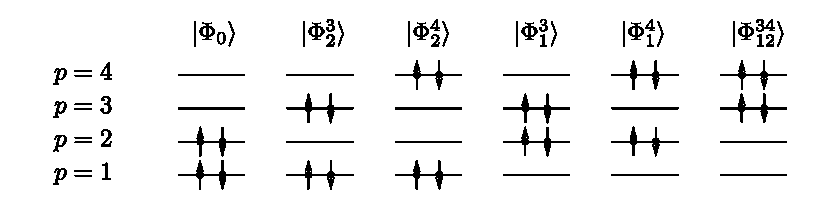
\includegraphics[width=\textwidth]{project2b.pdf}
	\caption{Sketch of the six possible Slater determinants. \label{fig:2}}
\end{figure}

These six Slater determinants are orthonormal and span a six-dimensional Hilbert space. We want to compute the matrix representation of the Hamiltonian in this space, which is given by
$$H_{ij} = \braopket{\Phi_i}{\op{H}}{\Phi_j},$$
where $\{\Phi_i\}_{i=1}^6$ is the set of the six Slater determinants. To calculate the different matrix elements, it's easiest to split up the Hamiltonian, so we have
$$H_{ij} = \braopket{\Phi_i}{\op{H}_0}{\Phi_j} + \braopket{\Phi_i}{\op{V}}{\Phi_j}. $$

The one-body operator is
\begin{align*}
\sum_{p\sigma} (p-1)a_{p\sigma}^\dagger a_{p\sigma},
\end{align*}
so we see that the for the off-diagonal terms, the one-body contribution vanishes. For the diagonal terms we find
\begin{align*}
\braopket{\Phi^{12}}{\op{H}_0}{\Phi^{12}} &= 2, \qquad \braopket{\Phi^{12}}{\op{H}_0}{\Phi^{12}} = 4, \qquad \braopket{\Phi^{12}}{\op{H}_0}{\Phi^{12}} = 6, \\
\braopket{\Phi^{12}}{\op{H}_0}{\Phi^{12}} &= 6, \qquad \braopket{\Phi^{12}}{\op{H}_0}{\Phi^{12}} = 8, \qquad \braopket{\Phi^{12}}{\op{H}_0}{\Phi^{12}} = 10.
\end{align*}

For the two-body operator we have
\begin{align*}
\braopket{\Phi^{ij}}{\op{V}}{\Phi^{kl}} &= -\frac{g}{2}\sum_{pq}\braopket{0}{\op{P}_i \op{P}_j \op{P}^+_p \op{P}_q \op{P}^+_k \op{P}^+_l}{0}.
\end{align*}
There can be two, one or no non-coincidences between the Slater determinants. If there are two non-coincidences, we see that the matrix element vanishes as we can only remove one non-coincidence. If there is one non-coincidence we have
\begin{align*}
\braopket{\Phi^{ij}}{\op{V}}{\Phi^{ik}} &= -\frac{g}{2}\sum_{pq}\braopket{0}{\op{P}_i \op{P}_j \op{P}^+_p \op{P}_q \op{P}^+_i \op{P}^+_k}{0}.
\end{align*}
When we sum over $p$ and $q$, the only term that survives is the term were $p=j$ and $q=k$, all other terms vanish due to the orthogonality of the the Slater determinants, so we 

If there are no non-coincidences, we have
\begin{align*}
\braopket{\Phi^{ij}}{\op{V}}{\Phi^{ij}} &= -\frac{g}{2}\sum_{pq}\braopket{0}{\op{P}_i \op{P}_j \op{P}^+_p \op{P}_q \op{P}^+_i \op{P}^+_j}{0}
\end{align*}
The only terms that survive in the sums are now the terms were $p=q=i$ or $p=q=j$, so we get two terms contributing to the final result.

We can then set up the Hamiltonian matrix
\begin{align*}
\op{H} = \begin{pmatrix}
2 - g &  -g/2 & -g/2  & -g/2  & -g/2  & 0     \\
-g/2  & 4 - g & -g/2  & -g/2  & 0     & -g/2  \\
-g/2  & -g/2  & 6 - g &	0     & -g/2  & -g/2  \\              
-g/2  & -g/2  & 0     & 6 - g &	-g/2  & -g/2  \\                         
-g/2  &	0	  & -g/2  & -g/2  & 8 - g & -g/2  \\
0     &  -g/2 & -g/2  & -g/2  &  -g/2 & 10 - g 
\end{pmatrix}
\end{align*}

Numerically, we find the eigenvalues and eigenvectors
\begin{align*}
\lambda = 
\begin{pmatrix}
0.780 \\  9.364 \\  7.065 \\  5.000 \\  2.791 \\  5.000 
\end{pmatrix}, \qquad
V =
\begin{pmatrix}
0.972 &  -0.041 &  -0.104 &  -0.154 &  -0.136 &  0.004  \\
-0.185 &  -0.101 &  -0.014 &  -0.309 &  -0.927 &  0.008  \\
-0.089 &  -0.154 &  -0.170 &  -0.617 &  0.242 &  -0.691  \\
-0.089 &  -0.154 &  -0.170 &  -0.617 &  0.242 &  0.723  \\
-0.066 &  -0.271 &  -0.908 &  0.309 &  -0.046 &  -0.008  \\
0.026 &  -0.931 &  0.326 &  0.154 &  0.039 &  -0.004  \\
\end{pmatrix}.
\end{align*}

\begin{figure}[htpb]
	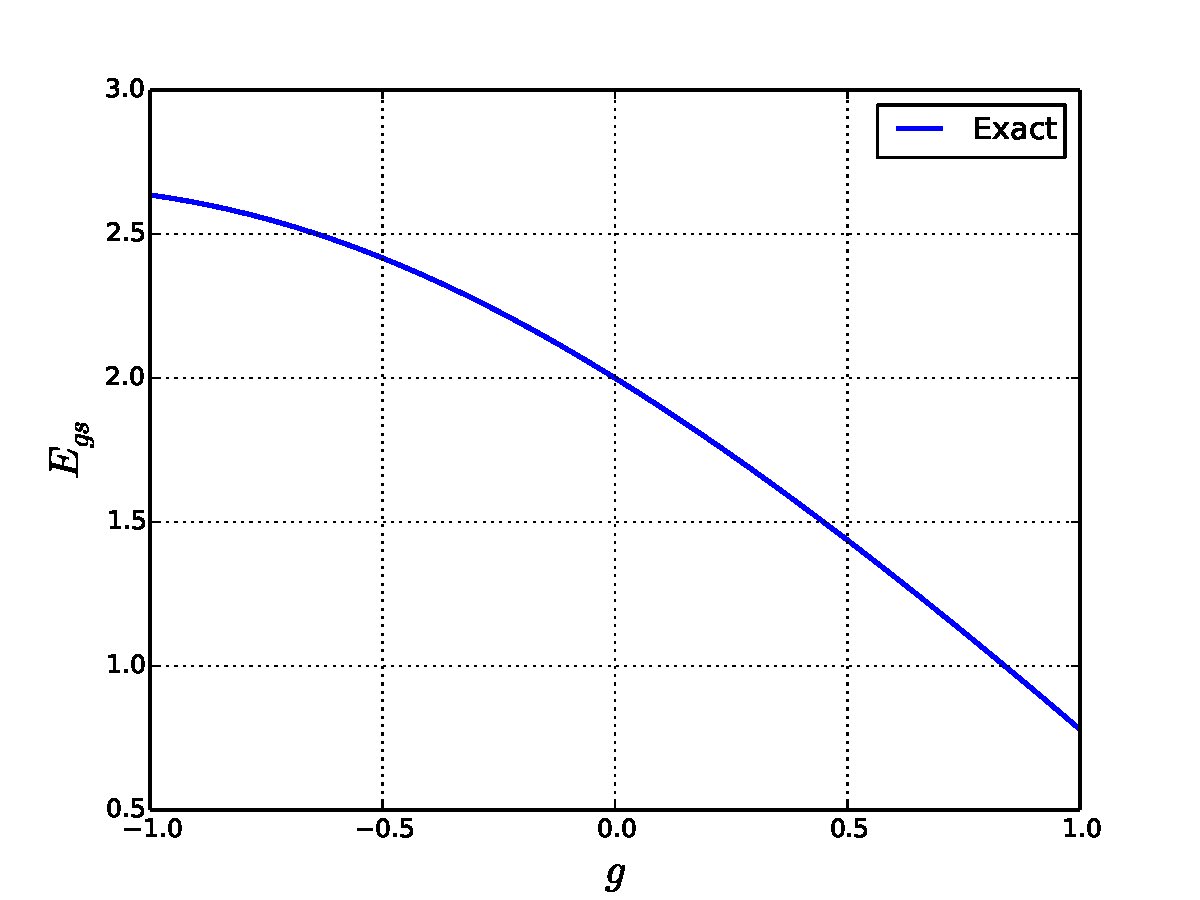
\includegraphics[width=\textwidth]{proj2_2.pdf}
	\caption{Ground state energy as a function of the interaction-parameter $g$. \label{fig:plot1}}
\end{figure}

\clearpage

\section*{Exercise 3)}

We now limit our system to at most two-particle-two-hole excitations. This means we discard $\ket{\Phi^{34}}$, and only look at a five-dimensional system.

The Hamiltonian matrix is then the five-by-five matrix
\begin{align*}
\op{H} = \begin{pmatrix}
2 - g &  -g/2 & -g/2  & -g/2  & -g/2  \\
-g/2  & 4 - g & -g/2  & -g/2  & 0     \\
-g/2  & -g/2  & 6 - g &	0     & -g/2  \\              
-g/2  & -g/2  & 0     & 6 - g &	-g/2  \\                         
-g/2  &	0	  & -g/2  & -g/2  & 8 - g \\
\end{pmatrix}
\end{align*}

\clearpage

\section*{Exercise 4)}

We now turn to Hartree-Fock theory, we will define our model space to consist of the single-particle levels $p=1,2$ and the excluded space is then $p=3,4$. This means we also define our reference state to be
$$\ket{\Phi_0} = \op{P}_1^+ \op{P}_2^+ \ket{0}.$$

The projection operator $\op{P}$ projects onto the model space, which is spanned by the reference function, so $\op{P} = \ket{\Phi_0}\bra{\Phi_0}$.


\subsection*{Partitioning the Hamiltonian}

If we limit ourselves to at most two-body interactions, the Hamiltonian can be generally written as a sum of one-body and two-body operators, which in second quantization looks like
$$\op{H} = \op{H}_1 + \op{H}_2 = \sum_\mu \op{h}_\mu + \sum_{\mu\nu} \op{v}_{\mu\nu}.$$
For our system we have a single one-body and a single two-body interaction, labeling them $\op{h}_0$ and $\op{v}$, we get
$$\op{H} = \sum_{\alpha\beta} \braopket{\alpha}{\op{h}_0}{\beta}\alpha^\dagger \beta + \frac{1}{4}\sum_{\alpha\beta\gamma\delta}\brakket{\alpha\beta}{\gamma\delta}\alpha^\dagger \beta^\dagger \delta \gamma,$$
where we use Shavitt and Bartlet's shorthand of $\brakket{\alpha\beta}{\gamma\delta} = \braopket{\alpha\beta}{\op{v}}{\gamma\delta}_{\rm AS}$.

Using Wick's theorem, we can write these out as 
\begin{align*}
\op{H}_1 &= \sum_{pq}\braopket{p}{\op{h}_0}{q}\{\op{p}^\dag \op{q}\} + \sum_{i}\braopket{i}{\op{h}_0}{i}, \\
\op{H}_2 &= \frac{1}{4}\sum_{pqrs} \brakket{pq}{rs} \{\op{p}^\dag \op{q}^\dag \op{s}\op{r}\} + \sum_{pqi} \brakket{pi}{qi} \{ \op{p}^\dag \op{q} \} + \frac{1}{2}\sum_{ij} \brakket{ij}{ij}.
\end{align*}
We now define the \emph{reference energy} as
$$E_{\rm ref} = \sum_{i}\braopket{i}{\op{h}_0}{i} + \frac{1}{2}\sum_{ij} \brakket{ij}{ij}.$$
Which enables us to split the Hamiltonian into its normal-ordered part and the reference energy
$$\op{H} = \op{H}_{\rm N} + E_{\rm ref}.$$
The normal-ordered Hamiltonian is then
$$\op{H}_{\rm N} = \sum_{pq}\braopket{p}{\op{h}_0}{q}\{\op{p}^\dag \op{q}\}  + \sum_{pqi} \brakket{pi}{qi}\{\op{p}^\dag \op{q}\}  + \frac{1}{4}\sum_{pqrs} \brakket{pq}{rs} \{\op{p}^\dag \op{q}^\dag \op{s}\op{r}\}.$$
We now relabel the first two terms into the normal-ordered \emph{Fock-operator}, giving us
$$\op{H}_{\rm N} = \op{F} + \frac{1}{4}\sum_{pqrs} \brakket{pq}{rs} \{\op{p}^\dag \op{q}^\dag \op{s}\op{r}\}.$$
We can now think of the normal-ordered Hamiltonian as the sum of a one-body part and the perturbation
$$\op{W}_{\rm N}  =\frac{1}{4}\sum_{pqrs} \brakket{pq}{rs} \{\op{p}^\dag \op{q}^\dag \op{s}\op{r}\},$$
we will get back to this when we turn to many-body perturbation theory.

\clearpage

For now, we will look closer at the normal-ordered Fock-operator
$$\op{F}_{\rm N} = \sum_{pq}\braopket{p}{\op{h}_0}{q}\{\op{p}^\dag \op{q}\}  + \sum_{pqi} \brakket{pi}{qi} \{\op{p}^\dag \op{q}\} = \sum_{pq} f_{pq} \{\op{p}^\dagger \op{q} \},$$
where
$$f_{pq} = \braopket{p}{\op{h}_0}{q} + \sum_{pqi} \brakket{pi}{qi} \{\op{p}^\dag \op{q}\} = h_{pq} + u_{pq}.$$
We see that the exact form of the Fock-matrix is then the result of the one-body and two-body operators $\op{h}_0$ and $\op{v}$ and also of our choice of single-particle basis. 

The form of the Fock-matrix is quite important for our further discussion of how to solve the problem, and so we will label three different general cases.
\begin{enumerate}
	\item First we have the possibility of the Fock-matrix being purely diagonal
	$$f_{pq} = \eps_p \delta_{pq},$$
	this case is known as the \emph{cannonical Hartree-Fock} case.
	\item Next, we have the case where the Fock-matrix is not entirely diagonal, but it is \emph{block-diagonal}, meaning the blocks of the Fock-matrix corresponding to the matrix elements between hole and particle states vanish. So we have
	$$f_{ai} = 0,$$
	this is the \emph{non-cannonical} Hartree-Fock case. Note that some people do not distinguish between the cannonical and non-cannonical HF cases.
	\item All cases not covered by the two HF cases are collectively reffered to as \emph{general} cases.
\end{enumerate}
As the normal-ordered Fock-operator can be non-diagonal, it is often conveniant to split it into its diagonal and off-diagonal contributions
$$\op{F}_{\rm N} = \sum_p f_{pp}\{\op{p}^\dagger \op{p}\} + \sum_{p\neq q} f_{pq}\{\op{p}^\dagger \op{q}\} = \op{F}_{\rm N}^{\rm D} + \op{F}_{\rm N}^{\rm O}.$$
In the cases where $\op{F}_{\rm N}^{\rm O} \neq 0$, it is common to include this part of the Fock-operator in the perturbation.

The total normal-product Hamiltonian is then
$$\op{H}_{\rm N} = \op{F}_{\rm N} + \op{W} = \op{F}^{\rm d}_{\rm N} + \op{F}^{\rm o}_{\rm N} + \op{W} = \op{F}^{\rm d}_{\rm N} + \mbox{(perturbation)}.$$

In our basis, we have
$$f_{pq} = \braopket{p}{\op{h}_0}{q}\{\op{p}^\dag \op{q}\}  + \sum_{i} \brakket{pi}{qi}\{\op{p}^\dag \op{q}\}.$$
Here the state indices run over both the quantum numberd $p$ and $\sigma$. As we have no $1p1h$-states, only $2p2h$-states, there will either be zero or two noncoincidences between states. This means that $\{\op{p}^\dag \op{q}\}$

\clearpage







$$\op{H} = \op{H}_0 + \op{V} = \sum_{p \sigma} (p-1)a_{p\sigma}^\dagger a_{p\sigma} 
 -\frac{1}{2}g \sum_{p q} a_{p+}^\dagger a_{p-}^\dagger a_{q-} a_{q+}.$$


\subsection*{Canonical and non-canonical Hartree-Fock}

For canonical Hartree-Fock, we now that the Fock-operator is diagonal, meaning
$$f_{pq} = \eps_p \delta_{pq}, \qquad \eps_p = h_{pp} + \sum_{i}\brakket{pi}{pi}.$$
For the non-canonical Hartree-Fock, the Fock-operator is a block-diagonal matrix, this means that $f_{ai}$ is zero, but $f_{ab}$ and $f_{ij}$ are generally not zero.
For the completely general case, there is no guarantee that any element of the Fock matrix is zero.
$$\op{H} = \sum_{pq} p^\dagger q + \frac{1}{4}\sum_{pqrs}\brakket{pq}{rs}p^\dagger q^\dagger s r.$$

\begin{align*}
\op{H}_0 &= \sum_{pq}\braopket{p}{\op{h}_0}{q}\{\op{p}^\dag \op{q}\} + \sum_{i}\braopket{i}{\op{h}_0}{i}, \\
\op{H}_1 &= \frac{1}{4}\sum_{pqrs} \braopket{pq}{\op{v}}{rs}_{\rm AS} \{\op{p}^\dag \op{q}^\dag \op{s}\op{r}\} + \sum_{pqi} \braopket{pi}{\op{v}}{qi}_{\rm AS} \{ \op{p}^\dag \op{q} \} + \frac{1}{2}\sum_{ij} \braopket{ij}{\op{v}}{ij}_{\rm AS}.
\end{align*}

We can then see that we have the Fock-operator
$$\op{F} = \sum_{pq} \braopket{p}{\op{h}_0}{q}\{\op{p}^\dagger\op{q}\} + \sum_{pqi} \brakket{p}{q}\{\op{p}^\dagger\op{q}\}.$$
So that the matrix elements of the Fock-matrix are given by
$$f_{pq} = h_{pq} + \sum_{i}\brakket{pi}{qi}.$$

We then have
$$\op{H} = \op{F} + \op{E}_{ref} + \frac{1}{4}\sum_{pqrs}\brakket{pq}{rs},$$
where
$$E_{ref} = \sum_i \braopket{i}{\op{h}_0}{i} + \frac{1}{2}\sum_{ij}\brakket{ij}{ij}.$$
So we have
$$\op{H}_{\rm N} = \op{F} + \frac{1}{4}\sum_{pqrs}\brakket{pq}{rs}.$$

If we are looking at canonical HF
$$f_{pq} = \eps_p \delta_{pq}.$$
If we are looking at non-canonical HF




\clearpage

\section*{Exercise 5)}

Diagram 3 vanishes due to the nature of the interaction.

Diagram 2 is only in non-can, diagram 6, 7, 6, 10, 11, 12, 13, 14, 15 and 16 all vanish.


\clearpage

We define the reference vacuum, which is our ansatz for the ground state $\ket{\Phi_0}$. We can define 1p-1h and 2p-2h excitations as $\op{T}_1\ket{\Phi_0}$ and $\op{T}_2\ket{\Phi_0}$.

We usually use the non-interacting part of the Hamiltonian as our single-particle wave functions.

We can then expand our exact ground state as

$$\ket{\Psi_0} = C_0\ket{\Phi_0} + \sum_{ai}C_i^a \ket{\phi_i^a} + \sum_{abij}C_{ij}^{ab}\ket{\Phi_{ij}^{ab}} + \ldots = (C_0 + \op{C})\ket{\Phi_0}.$$
Where we have introduced the correlation operators
$$\op{C} = \sum_{ai}C_i^a \op{a}_{a}^\dagger \op{a}_i  + \sum_{abij}C_{ij}^{ab} \op{a}_{a}^\dagger \op{a}_{b}^\dagger \op{a}_j \op{a}_i $$

We now set $C_0 = 1$, giving
$$\ket{\Psi_0} = (1+\op{C})\ket{\Phi_0}.$$
$$\ket{\Psi_0} = \sum_{PH} C_{H}^P \Phi_H^P.$$

For all PH sets we get
$$\sum_{P'H'} \braopket{\Phi_H^P}{\op{H}-E}{\Phi_{H'}^{P'}} = 0.$$

In Perturbation theory we assume that the exact ground state wave function is dominated by $\ket{\Phi_0}$ and can be written in intermediate normalization as
$$\ket{\Psi_0} = \ket{\Phi_0} + \sum_{m=1}^\infty C_m \ket{\Phi_m}.$$
From the Schrödinger equation, we have
$$\braopket{\Phi_0}{\op{H}}{\Psi_0} = E,$$
And
$$\braopket{\Psi_0}{\op{H}_0}{\Phi_0} = W_0,$$
so we can define
$$\Delta E = E - W_0 = \braopket{\Phi_0}{\op{H}_I}{\Psi_0}.$$
This quantity is called the correlation energy.

$$\op{P} = \ketbra{\Phi_0}{\Phi_0},$$
$$\op{Q} = \sum_{m=1}^\infty \ketbra{\Phi_m}{\Phi_m}.$$
$$\ket{\Psi_0} = (\op{P} + \op{Q})\ket{\Psi_0} = \ket{\Phi_0} + \op{Q}\ket{\Psi_0}.$$

$$\chi_n = \ket{\Psi_n} - \ket{\Phi_n}.$$
$$\braket{\Phi_n}{\Phi_n} = 1, \quad \braket{\Psi_n}{\Phi_n} = 1, \quad \braket{\chi_n}{\Phi_n} = 0, \quad \braket{\Psi_n}{\Psi_n} = 1 + \braket{\chi_n}{\chi_n}.$$

Idempotenence
$$\op{P}^2 = \op{P}, \quad \op{Q}^2 = \op{Q}$$
$$\op{P}\op{Q} = 0. $$

The operator $\op{P}$ projects the component of $\Psi$ that is parallel to $\Phi_0$, which can be seen from
$$\op{P}\Psi = \sum_{a_i}\ketbra{\Phi_0}{\Phi_0}\ket{\Phi_i} = a_0\ket{\Phi_0}.$$
While $\op{Q}$ annihilates the $\Phi_0$ component, leaving everything else intact. This also means that
$$\Psi = (\op{P} + \op{Q})\Psi.$$

\clearpage

\section*{Exercise 7)}

\subsubsection*{Linked and unlinked diagrams}

A diagram is called unlinked if and only if it has a disconnected part that is closed, meaning it has no open lines.


Goldstones linked-diagram theorem states that all unliked diagrams will cancel agains the renormalization terms in RSPT, meaning we can express the energy and wave function in each order as a sum of linked diagrams only \footnote{See Shavitt and Bartlet section 5.8.}. This means we have

\clearpage

In general, we have
$$\big(E^{(0) - \op{H}}\big) \Psi^{(m)} = (E^{(1)}-\op{V})\Psi^{(m-1)} - \sum_{l=0}^{m-1} E^{m-l}\Psi^{(l)}.$$
We can apply $\bra{\Phi}$ to the equation and find
$$E^{(m)} = \braopket{\Phi}{\op{V}}{\Psi^{(m-1)}}.$$

As $\xi$ is only a scalar that is multiplied with $H_0$, and we already the scaling $g$, we can se the parameter $\xi$ equal to 1, without a loss of generality.

Decompose the solution into
$$\Psi = (\op{P} + \op{Q})\Psi = \op{P}\Psi + \op{Q}\Psi = \Phi + \chi.$$

\begin{align*}
\Psi = \sum_{m=0}^\infty \big[\op{R_0}(\op{V}-\op{E}) \big]^m \Phi, \\
\Delta E = \sum_{m=0}^\infty \braopket{\Phi}{\op{V}\big[\op{R_0}(\op{V}-\op{E}) \big]^m}{\Phi}
\end{align*}


Cannonical HF
$$f_{pq} = \eps_p \delta_{pq}$$
$$\eps_p = h_{pp} + \sum_{i} \brakket{pi}{pi}.$$

Non-cannonical HF
$$f_{ia} = 0.$$

Fock-operator
$$\op{F} = \sum_{pq} f_{pq}\op{p}^\dagger \op{q}.$$
$$\op{U} = \sum_{pq} u_{pq}\op{p}^\dagger \op{q}.$$

$$\op{F} = \op{H}_0 + \op{U} = \sum_{pq} (h_{pq} + u_{pq})\op{p}^\dagger \op{q}.$$
$$\op{u} = \sum_i (\op{J}_i - \op{K}_i).$$

The normal-product Schrodinger equation is
$$\op{H}_{\rm N} \Psi = \Delta E \Psi,$$
where $\Delta E$ is the correlation energy in the Hartree-Fock case, the normal-product Hamiltonian is
$$\op{H}_{\rm N} = \op{F}_{\rm N} + \op{W} = \op{F}^d_{\rm N} + \op{F}^o + \op{W} = \op{F}^d + \op{V}_{\rm N}.$$


\end{document}